%% DONE
\id{IRSTI 06.52.17}{https://doi.org/10.58805/kazutb.v.1.26-782}

\begin{articleheader}
\sectionwithauthors{A. Galymzhanova, S. Singh, Sh. Sarkambayeva, A. Boranbayeva, A.Zh. Turegeldinova}{CHALLENGES AND OPPORTUNITIES IN MANAGING SMART CITY PROJECTS: A CASE STUDY OF KAZAKHSTAN' S URBAN TRANSFORMATION}

{\bfseries
\textsuperscript{1}A. Galymzhanova\alink{https://orcid.org/0009-0006-0462-2917},
\textsuperscript{2}S. Singh\alink{https://orcid.org/0000-0002-7707-031X},
\textsuperscript{3}Sh. Sarkambayeva\textsuperscript{\envelope } \alink{https://orcid.org/0000-0001-8509-3688},
\textsuperscript{1}A. Boranbayeva\alink{https://orcid.org/0000-0001-7239-9581},
\textsuperscript{3}A.Zh. Turegeldinova\alink{https://orcid.org/0000-0003-1042-1530}}
\end{articleheader}

\begin{affiliation}
\emph{\textsuperscript{1}Kazakh National University named after al-Farabi, Almaty, Kazakhstan,}

\emph{\textsuperscript{2}University of Fiju, Republic of Fiju,}

\emph{\textsuperscript{3}Kazakh National Research Technical University named after K.I. Satpayev, Almaty, Kazakhstan,}

\raggedright \textsuperscript{\envelope }{\em Correspondent-author: \href{mailto:sh.sarkambayeva@satbayev.university}{\nolinkurl{sh.sarkambayeva@satbayev.university}}}
\end{affiliation}

The article discusses the problems and opportunities of introducing
smart city technologies in Kazakhstan through the prism of project
management. Key aspects such as infrastructure quality, sustainable
\\development, data protection, citizen participation, government support
and the introduction of innovative technologies are analyzed. Examples
of successful projects in Kazakhstan, such as transport and lighting
management systems, as well as the experience of international
practices, including Singapore and Germany, are given.

The study highlights the importance of integrating sustainable
solutions, reducing digital inequality, and ensuring citizen
participation in digitalization processes. In addition, the need to
adapt international models of project management to the socio-economic
and cultural characteristics of Kazakhstan is noted. Quantitative and
qualitative analysis methods are used, including surveys, expert
interviews and data \\visualization, which allows us to identify the
interrelationships between various aspects of the \\implementation of
smart city projects.

The practical significance of the article lies in the development of
recommendations for public and private organizations aimed at improving
the effectiveness of stakeholder interaction, stimulating citizen
participation in digital transformation and creating conditions for
sustainable urban development. The findings of the study can serve as a
basis for strategic planning and decision-making in the field of smart
city project management in Kazakhstan.

{\bfseries Keywords: s}mart cities, project management, urban
transformation, Kazakhstan, sustainable \\development, governance models,
technological innovation, stakeholder collaboration, public-private\\
partnerships.

\begin{articleheader}
{\bfseries "АҚЫЛДЫ ҚАЛА" ЖОБАЛАРЫН БАСҚАРУДАҒЫ ҚИЫНДЫҚТАР МЕН МҮМКІНДІКТЕР: ҚАЗАҚСТАННЫҢ ҚАЛАЛЫҚ ТРАНСФОРМАЦИЯСЫНЫҢ ЖАҒДАЙЛЫҚ ЗЕРТТЕУІ}

{\bfseries
\textsuperscript{1}A. Ғалымжанқызы,
\textsuperscript{2}С. Сингх,
\textsuperscript{3}Ш. Сарқамбаева\textsuperscript{\envelope },
\textsuperscript{1}A. Боранбаева,
\textsuperscript{3}A.Ж. Төрегелдинова}
\end{articleheader}

\begin{affiliation}
\emph{\textsuperscript{1}Әл-Фараби атындағы Қазақ Ұлттық Университеті, Алматы, Казақстан,}

\emph{\textsuperscript{2}Фиджи университеті, Фиджи Республикасы,}

\emph{\textsuperscript{3}Қ.И. Сәтбаев атындағы Қазақ Ұлттық Техникалық Зерттеу Университеті, Алматы, Казақстан,}

\emph{e-mail: \href{mailto:sh.sarkambayeva@satbayev.university}{\nolinkurl{sh.sarkambayeva@satbayev.university}}}
\end{affiliation}

Мақалада жобалық басқару призмасы арқылы Қазақстанда ақылды қала
технологияларын енгізу мәселелері мен мүмкіндіктері қарастырылады.
Инфрақұрылымның сапасы, орнықты даму, деректерді қорғау, азаматтардың
қатысуы, мемлекетті қолдау және инновациялық технологияларды енгізу
сияқты негізгі аспектілер талданады. Қазақстанда көлік пен
жарықтандыруды басқару жүйелері сияқты табысты жобалардың мысалдары,
сондай-ақ Сингапур мен Германияны қоса алғанда, халықаралық
тәжірибелердің тәжірибесі келтіріледі.

Зерттеу тұрақты шешімдерді біріктірудің, цифрлық теңсіздікті
төмендетудің және азаматтардың цифрландыру процестеріне қатысуын
қамтамасыз етудің маңыздылығын көрсетеді. Бұдан басқа, жобалық
басқарудың халықаралық модельдерін Қазақстанның әлеуметтік-экономикалық
және мәдени ерекшеліктеріне бейімдеу қажеттілігі атап өтіледі. Сандық
және сапалық талдау әдістері, соның ішінде сауалнамалар, сараптамалық
сұхбаттар және деректерді визуализациялау қолданылады, бұл ақылды қала
жобаларын жүзеге асырудың әртүрлі аспектілері арасындағы байланысты
анықтауға мүмкіндік береді.

Мақаланың практикалық маңыздылығы мүдделі тараптардың өзара іс-қимылының
тиімділігін арттыруға, азаматтардың цифрлық трансформацияға қатысуын
ынталандыруға және тұрақты қала дамуы үшін жағдай жасауға бағытталған
мемлекеттік және жеке ұйымдар үшін ұсынымдар әзірлеу болып табылады.
Зерттеу қорытындылары Қазақстандағы ақылды қалалардың жобаларын басқару
саласында стратегиялық жоспарлау мен шешім қабылдау үшін негіз бола
алады.

{\bfseries Түйін сөздер:} ақылды қалалар, жобаларды басқару, қалаларды
трансформациялау, Қазақстан, тұрақты даму, басқару модельдері,
технологиялық инновациялар, мүдделі тараптардың ынтымақтастығы,
мемлекеттік-жекеменшік әріптестік.

\begin{articleheader}
{\bfseries ПРОБЛЕМЫ И ВОЗМОЖНОСТИ В УПРАВЛЕНИИ ПРОЕКТАМИ "УМНОГО ГОРОДА": НА ПРИМЕРЕ ТРАНСФОРМАЦИИ ГОРОДОВ КАЗАХСТАНА}

{\bfseries
\textsuperscript{1}A. Галымжанова,
\textsuperscript{2}С. Сингх,
\textsuperscript{3}Ш Саркамбаева\textsuperscript{\envelope },
\textsuperscript{1}A. Боранбаева,
\textsuperscript{3}A.Ж. Турегельдинова}
\end{articleheader}

\begin{affiliation}
\emph{\textsuperscript{1}Казахский национальный университет имени аль-Фараби, Алматы, Казахстан,}

\emph{\textsuperscript{2} Университет Фиджи, Республика Фиджи,}

\emph{\textsuperscript{3}Казахский национальный исследовательский технический университет имени К.И. Сатпаева, Алматы, Казахстан,}

\emph{e-mail: \href{mailto:sh.sarkambayeva@satbayev.university}{\nolinkurl{sh.sarkambayeva@satbayev.university}}}
\end{affiliation}

В статье рассматриваются проблемы и возможности внедрения технологий
умного города в Казахстане через призму проектного управления.
Анализируются ключевые аспекты, такие как качество инфраструктуры,
устойчивое развитие, защита данных, участие граждан, поддержка
государства и внедрение инновационных технологий. Приводятся примеры
успешных проектов в Казахстане, таких как системы управления транспортом
и освещением, а также опыт международных практик, включая Сингапур и
Германию.

Исследование подчеркивает важность интеграции устойчивых решений,
снижения цифрового неравенства и обеспечения участия граждан в процессах
цифровизации. Кроме того, отмечается необходимость адаптации
международных моделей проектного управления к социально-экономическим и
культурным особенностям Казахстана. Используются методы количественного
и качественного анализа, включая опросы, экспертные интервью и
визуализацию данных, что позволяет выявить взаимосвязи между различными
аспектами реализации проектов умных городов.

Практическая значимость статьи заключается в разработке рекомендаций для
государственных и частных организаций, направленных на повышение
эффективности взаимодействия заинтересованных сторон, стимулирование
участия граждан в цифровой трансформации и создание условий для
устойчивого городского развития. Выводы исследования могут служить
основой для стратегического планирования и принятия решений в области
управления проектами умных городов в Казахстане.

{\bfseries Ключевые слова:} умные города, управление проектами, городская
трансформация, Казахстан, устойчивое развитие, модели управления,
технологические инновации, сотрудничество с заинтересованными сторонами,
государственно-частное партнерство.

\begin{multicols}{2}
{\bfseries Introduction.} Digital transformation of cities is an essential
component of sustainable development, and its implementation through
project management is the key to improving the efficiency and quality of
the urban environment. With increasing urbanization and the need to
optimize resource management, Kazakhstan is striving to create smart
cities that integrate digital technologies to improve the quality of
life, sustainability, and economic development.

The concept of a "smart city" has become an important part of the
strategy for the development of cities around the world in recent
decades. It involves the use of innovative technologies such as the
Internet of Things (IoT), big data, blockchain and artificial
intelligence to improve the quality of life, increase economic
efficiency and ensure the sustainability of urban systems. In
Kazakhstan, elements of a smart city include intelligent transport
management projects, automated utility systems and e-government. For
example, in Astana, the Smart Astana program is being implemented, which
covers intelligent lighting, parking management and digitalization of
public services.

However, the introduction of such technologies requires not only
significant financial resources, but also high-quality project
management. For Kazakhstan, where the process of transformation from a
post-Soviet management system to a modern one is underway, this
direction is especially relevant, since it intersects with the tasks of
increasing transparency, strengthening citizens'{} trust
and sustainable development.

According to McKinsey, cities that have implemented digital solutions
can improve the quality of life of citizens by 10-30\% by reducing
emissions, improving safety and improving transport accessibility. Smart
cities also contribute to sustainable development -- they provide
improved energy management, which can reduce energy consumption by
15-25\% {[}1{]}.

According to UN DESA, global investments in smart cities amount to about
\$124 billion and continue to grow by 18-20\% annually. Kazakhstan,
which actively attracts international investments, needs effective
project management models to ensure sustainability and integration of
innovations into the urban environment {[}2{]}.

According to the World Bank, the level of urbanization in Kazakhstan
reached approximately 58\% in 2023, reflecting the rapid growth of the
urban population and the need to modernize urban infrastructure.
Forecasts show that by 2030 this figure could rise to 65\%, which
creates a serious burden on urban systems and increases the need for
sustainable solutions {[}3{]}.

In 2017, Kazakhstan adopted the Digital Kazakhstan program aimed at
digitalization of all spheres, including urban governance. However,
successful implementation requires design approaches that take into
account complex challenges such as security, sustainable use of
resources, digital inequality and public participation {[}4{]}.

According to UN reports, cities generate more than 70\% of global CO₂
emissions, and in Kazakhstan, greenhouse gas emissions also remain high
due to the dominance of traditional energy. The use of smart city
technologies, such as smart energy systems, can reduce emissions by
15-20\%, which is in line with Kazakhstan' s sustainable
development goals to reduce its carbon footprint.

According to IHS Markit estimates, global investments in smart cities
will amount to more than \$327 billion by 2025, and this area continues
to develop rapidly. Kazakhstan is actively attracting investors, and
projects within the framework of smart cities can increase capital
inflows, as well as create up to 100,000 new jobs related to IT and
engineering in the next 10 years.

According to the OECD, about 40\% of Kazakhstanis in rural areas still
do not have stable access to high-speed Internet, which is an obstacle
to the full implementation of digital solutions. Eliminating digital
inequality in cities and minimizing it in suburban areas are important
aspects for successful digital transformation.

Pilot smart city projects have already been initiated in Uzbekistan and
Kazakhstan, including projects on transport management and street
lighting, which have shown an improvement in reducing energy consumption
by 25\% and reducing congestion by 10-15\% in Almaty. The expansion of
such projects, with the support of integrated project management, will
allow Kazakhstan to take a leading position in digital transformation
among the countries of Central Asia.

The main research question is formulated as follows: \emph{How can
international approaches to smart city project management be adapted for
implementation in Kazakhstan, taking into account its socio-economic,
cultural and infrastructural features?}

The purpose of the research is to analyze the problems and opportunities
that arise in the process of implementing smart city projects in
Kazakhstan, as well as to develop recommendations for adapting
international smart city project management models in order to increase
their efficiency and sustainability in Kazakhstan cities.

The object of the study is the processes of smart city project
management, including the introduction of innovative technologies and
management systems into urban infrastructure, as well as their
adaptation in the conditions of Kazakhstan.

The scientific novelty of this study lies in a systematic approach to
analyzing problems and opportunities in the context of the specific
realities of Kazakhstan, which allows for a deeper understanding of the
specific barriers and opportunities for the successful implementation of
smart cities in developing countries. The study also expands existing
approaches in project management, offering additional strategies and
recommendations for effective management of digitalization processes and
sustainable urban development.

The practical value of the research lies in the development of proposals
for public and private organizations that are engaged in the design and
implementation of smart city initiatives. The proposed recommendations
will help improve interaction between stakeholders, stimulate citizen
participation in the digital transformation process and create
conditions for sustainable urban development. It also contributes to
improving the social and environmental sustainability of urban spaces
and increasing the quality of life of citizens.

\emph{Literature Review.} In order to improve the quality of life for
its inhabitants and handle the complexity of persistent issues with
urban settings, smart city initiatives are being supported globally
{[}5{]}. Additionally, cities are being pressured to fulfill their part
in tackling new global issues including resilience {[}6{]},
decarbonization {[}7{]}, and sustainability {[}8{]}. The creation of
more sustainable infrastructure, new transportation paradigms
{[}9,10{]}, smart urbanism {[}11{]}, public participation {[}12,13{]},
municipal governance {[}14{]}, or sustainability {[}15{]} are only a few
of the many areas of activity that are included in smart city efforts.
In terms of their goals, innovative methodologies, key technologies,
priorities, or the characteristics of the urban environments in which
they are implemented, these programs can take many different forms.
Nevertheless, they all agree that digital technologies have the capacity
to revolutionize urban life and serve as the primary facilitator for a
constructive, forward-thinking, and long-lasting influence {[}16{]}.

Nonetheless, there are indications of dissatisfaction with the tangible
results of smart city projects {[}17,18{]} as well as opposition to what
is increasingly thought to be an overabundance of corporate control over
technology in urban areas {[}19{]}. Regardless of one' s
overall political stance on smart cities, it appears reasonable to
acknowledge that, thus far, the actual outcomes may be viewed as being
rather constrained in relation to the corresponding investments and the
stated aspirations. More precisely, it becomes evident from the
standpoint of digital innovation that the rate of invention is
substantially slower than in other fields where important
characteristics of digital innovation, including generativity and
convergence, have sparked swift and profoundly disruptive changes
{[}20{]}.

Trindade et al. {[}21{]} discussed the connection between the ideas of
smart cities and sustainability, arguing that the latter can be
effectively facilitated by the former as a concept and set of
activities. In order for future investments to be justified by
socioeconomic needs and environmental concerns rather than technological
advancement and industrial competitiveness, Bibri and Krogstie {[}22{]}
emphasize the necessity of connecting the development and innovation of
information and communication technology (ICT) with sustainable
development. According to Yigitcanlar et al. {[}8{]}, cities cannot be
smart unless they are sustainable. They explain a conflict between the
objectives of sustainable urban development and the shared dreams of
smart cities. Bibri {[}23{]} emphasizes the potential for using big data
analytics to meet sustainable development objectives, but she also
recommends that researchers concentrate more on pinpointing practical
problems and specific knowledge gaps. Ramaswami et al. {[}15{]} also
discuss this link between data science and urban sustainability, arguing
that smart city programs need to go beyond city-level data to a
higher-order understanding of cities as transboundary systems with a
variety of players, priorities, and solutions. A review by Ben Letaifa
{[}24{]} indicates that when developing plans for smart cities, macro,
mezzo, and micro aspects should be taken into account. It also offers a
methodological framework for the implementation of smart cities.

Meijer and Bolívar' s review {[}14{]} discusses smart
city administration. From straightforward institutional arrangements to
more radical conceptualizations where the government itself must be
changed to create a smart city, the authors identify various
conceptualizations of smart city governance that vary in the degree of
government transformation required to make cities smarter. Of the 20
drivers for smart city innovation and their prioritization identified in
the analysis by Guedes et al. {[}25{]}, 15 are mostly concerned with
city government, while the remaining 5 are related to technology.

In order to better comprehend the difficulties faced by smart city
programs, we examine a digital innovation lens in this study. In order
to determine if smart city projects can truly create an environment of
open and flexible affordances that fosters innovations that are
characterized by convergence and generativity, we expand on the
essential features of digital technology as suggested by Yoo et al.
{[}20{]}. Understanding how much the primary obstacles to smart city
initiatives might all be distinct expressions of a single issue stemming
from a misalignment between smart city innovation practices and the
fundamental ideas that drove digital innovation' s rapid
success in other fields is the main driving force.

According to a study published in the MDPI Smart Cities journal, smart
cities use digital technologies and data analysis to improve the quality
of life of citizens, improve the efficiency of infrastructure and
services, and stimulate sustainable economic growth. The review examined
the definition of smart cities, their advantages and disadvantages, as
well as key implementation challenges, including issues of data privacy
and digital inequality.

Research at IEEE Xplore analyzes key challenges and opportunities in
smart city project management. Special attention is paid to the need for
an integrated management approach that unites the public and private
sectors. Among the main challenges are shortcomings in the regulatory
framework, financial instability and poor coordination between
stakeholders.

Other researches have noted that smart cities contribute to achieving
sustainable development goals, including reducing carbon dioxide
emissions, improving energy efficiency and improving transport
accessibility. However, issues such as digital inequality and
cybersecurity remain relevant.

Agueda Veloso, Fernando Fonseca, Ru Ramos (2024) analyze examples of the
implementation of smart cities in Singapore, Barcelona, Helsinki and
Medellin. The main focus is on sustainable development, where it is
noted that most projects focus on management and environmental aspects.
The study highlights the need for more holistic approaches to address
the complex challenges of urbanization and the introduction of
standardized assessment methods {[}26{]}.

An analysis of the existing literature shows that smart city project
management is a complex interdisciplinary field that requires the
integration of technology, sustainable development, social participation
and effective management. Research by foreign authors (Giffinger et al.,
Komninos, Allam) focuses on the general concepts of smart cities, such
as technology adoption, urban sustainability and public participation
{[}27{]}. They emphasize the importance of strategic planning and the
availability of criteria for evaluating the effectiveness of smart
cities.

Kazakh literature, on the contrary, focuses on the practical aspects of
the implementation of the Digital Kazakhstan program and local
challenges. The main problems include a lack of resources, poor
coordination between agencies, digital inequality, and low
infrastructure availability.

A significant gap is the lack of unified approaches to managing smart
city projects adapted to the conditions of Kazakhstan. Foreign studies
offer examples of successful management models, but they require
localization. Also, insufficient attention is paid to the integration of
innovations into the social sphere, which is critically important for
Kazakhstan with its high degree of urbanization.

Thus, further research should be aimed at developing adapted smart city
project management models that take into account local challenges and
international experience. This will create the basis for the sustainable
and inclusive development of the urban environment.

The process of implementing smart city projects in Kazakhstan faces a
number of problems, such as insufficient coordination between various
public and private institutions, lack of qualified personnel,
insufficient financing and technical immaturity of infrastructure. These
problems create barriers to the effective implementation of innovative
solutions in the urban environment and hinder the development of
sustainable and smart cities, which requires the development of adapted
project management models to improve management and ensure the
sustainability of these projects in Kazakhstan.

{\bfseries Materials and methods.} The study used methods of qualitative
and quantitative analysis to study the problems and opportunities of
smart city project management using the example of Kazakhstan.
Interviews with experts, surveys of urban residents on their readiness
to implement smart technologies, as well as an analysis of existing
literature with an emphasis on local and international features were
used to collect data. Additionally, a case method was used to analyze
implemented projects, and a comparative analysis made it possible to
compare successful initiatives of Kazakhstan with international
experience. The data was processed using graphical visualization,
including the construction of histograms, pie charts and tables, which
made it possible to classify and rank key categories such as
infrastructure, sustainable development, data security, digital
inequality, government support and innovative technologies. This
approach provided an in-depth analysis and identification of the
interrelationships between various aspects of the implementation of
smart city projects.

{\bfseries Results and discussions.} Various methods suitable for the
analysis of both qualitative and quantitative data were used to study
the problem "Problems and opportunities in the management of smart City
projects: on the example of the transformation of cities in Kazakhstan".
The methods include interviews with experts, questionnaires, comparative
analysis, case-stage method and analysis of existing literature. The
following techniques were used to collect, process and analyze data.

A histogram showing the readiness of residents of different cities of
Kazakhstan to implement intelligent technologies. The chart shows the
percentage of respondents who are ready to implement smart city
solutions in each city. Figure 1 shows the proportion of respondents who
said that they were prepared to implement smart city technology from
five different cities: Almaty, Nur-Sultan, Shymkent, Karaganda, and
Aktobe. With 50\% of respondents indicating a readiness to adopt smart
city solutions, Aktobe has the highest rate among these cities. At 45\%,
Shymkent comes in second, showing a high level of preparation as well.

At 40\%, Almaty, a significant Kazakh city, exhibits a moderate level of
preparedness. The capital city of Nur-Sultan, on the other hand, has a
somewhat lower ratio of 35\%, indicating a less enthusiastic but still
noticeable preference for smart city efforts. However, only 30\% of
respondents said they were in favor of using such technologies, making
Karaganda the least prepared city in the study.

These discrepancies can be the result of disparities in local government
initiatives, municipal infrastructure, public understanding of the
advantages of smart cities, and technology accessibility. While places
like Karaganda could need more focused efforts to raise awareness and
readiness, communities like Aktobe and Shymkent might have customized
programs or favorable settings that spark greater enthusiasm.
\end{multicols}

\begin{figure}[H]
	\centering
	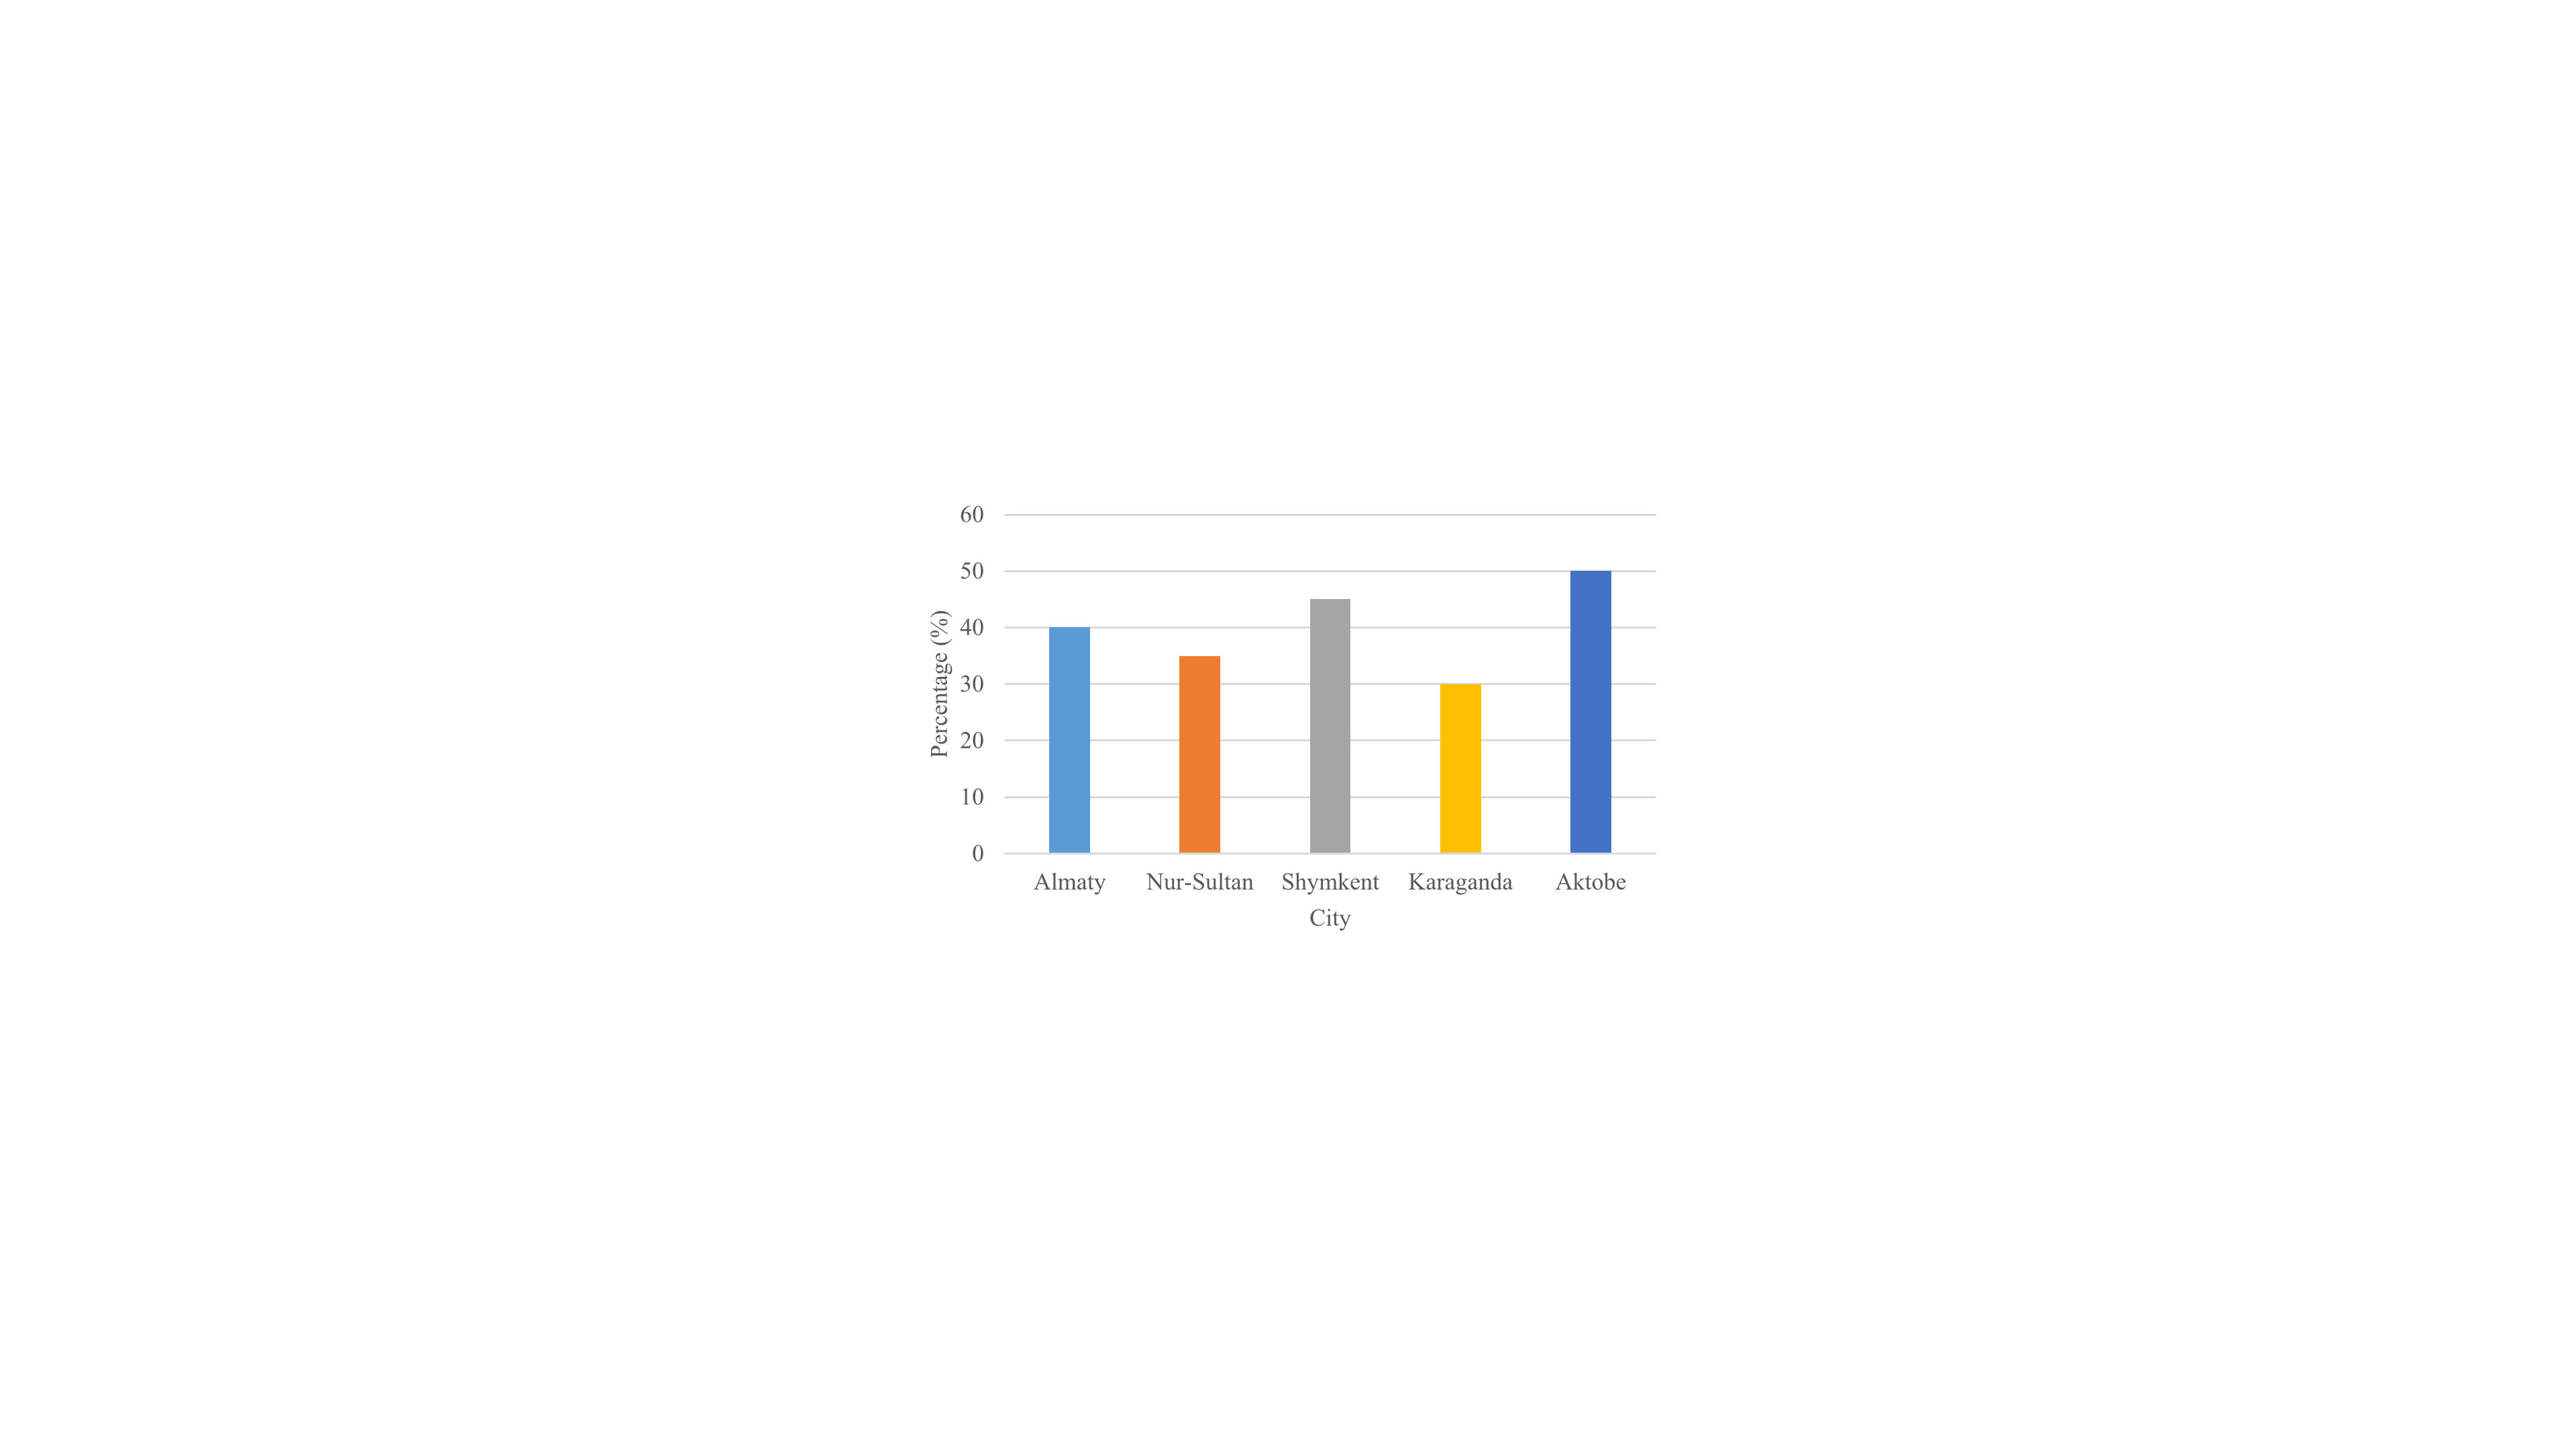
\includegraphics[width=0.7\textwidth]{media/ekon/Graph_12}
	\caption*{Fig. 1 - The percentage of respondents who said that they were prepared to implement smart city technology}
	\caption*{\normalfont \emph{(compiled by the authors based on {[}28{]})}}
\end{figure}

\begin{multicols}{2}
Figure 2 shows a prioritizing of features depending on respondent
preferences, highlighting the perceived relevance of different parts of
smart cities. With 30\% of respondents highlighting its significance,
security stands out as the most important factor. This illustrates how
safety, which includes emergency response systems, crime prevention
technology, and surveillance systems, is widely acknowledged as a
fundamental component of smart cities.
\end{multicols}

\begin{figure}[H]
	\centering
	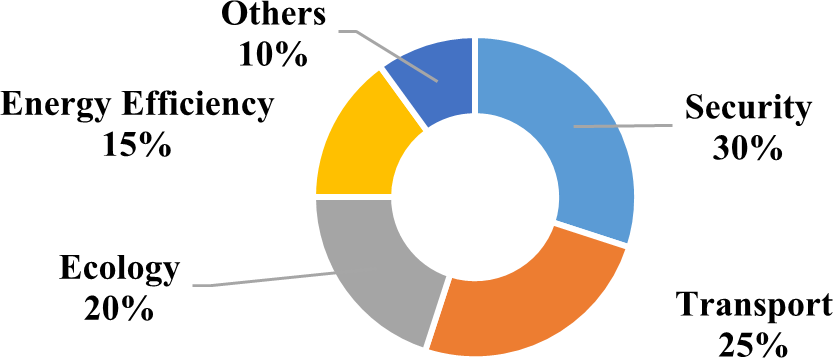
\includegraphics[width=0.6\textwidth]{media/ekon/Graph_13}
	\caption*{Fig. 2 - Prioritizing of features depending on respondent preferences}
	\caption*{\normalfont \emph{(compiled by the authors based on {[}28{]})}}
\end{figure}

\begin{multicols}{2}
Transport received 25\% of the replies, making it the second most
important factor. Enhancing mobility and lowering urban congestion, a
major issue for many cities, requires sophisticated and efficient
transportation systems, such as integrated public transit options and
real-time traffic management.

With 20\% of respondents emphasizing its importance, ecology comes in
third. In order to solve environmental issues and guarantee a higher
standard of living, smart city solutions aimed at ecological
sustainability such as waste management, air quality monitoring, and
green urban planning are essential.

15\% of respondents said that energy efficiency was a top priority,
which is consistent with the increased focus on lowering energy use
through the use of smart grids and energy-efficient infrastructure. Both
environmental preservation and economic viability depend on this factor.

Lastly, 10\% of respondents said that other factors such as governance,
healthcare, education, and cultural initiatives were important. Despite
getting less emphasis, these components support a smart
city' s overall growth.

In order to produce secure, effective, and livable urban places, the
data highlights the complexity of smart city development and the
necessity to balance security, mobility, ecological sustainability,
energy efficiency, and other factors.

The number of successful smart city initiatives in the USA, Germany,
Singapore, South Korea, and Kazakhstan is shown in Figure 3. The
information highlights Kazakhstan' s comparative position
and offers insight into the adoption and execution of smart city
programs worldwide.

With 12 successful smart city initiatives, the USA leads the world and
demonstrates its leadership in implementing cutting-edge urban
technologies. These initiatives, which are supported by significant
expenditures and a robust innovation environment, probably include a
range of topics, including energy management, smart transportation, and
security systems.

Germany comes in second with ten projects, demonstrating its focus on
fusing environmental principles with smart technology. In keeping with
its larger commitment to environmental sustainability, Germany
frequently uses smart grids, eco-friendly urban planning, and green
infrastructure.
\end{multicols}

\begin{figure}[H]
	\centering
	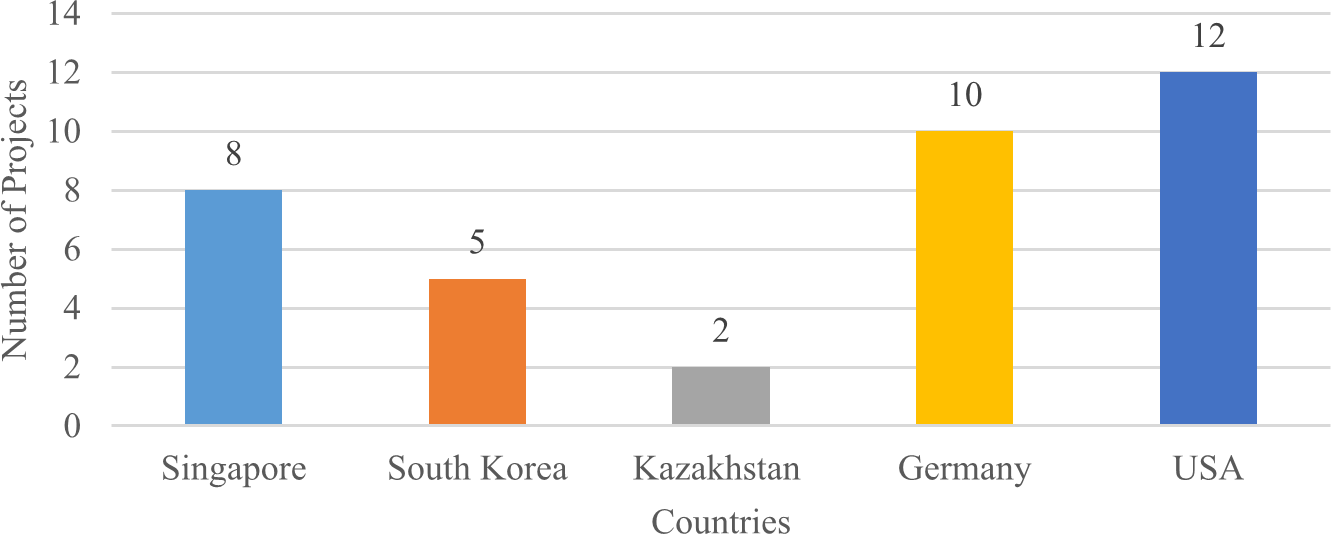
\includegraphics[width=0.8\textwidth]{media/ekon/Graph_14}
	\caption*{Fig. 3 - The number of successful smart city initiatives in the USA, Germany, Singapore, South Korea, and Kazakhstan}
	\caption*{\normalfont \emph{(compiled by the authors based on {[}28{]})}} 
\end{figure}

\begin{multicols}{2}
With eight initiatives, Singapore is a prime example of a tiny yet
incredibly effective smart city deployment approach. Singapore, which is
well-known for its extensive Smart Nation effort, positions itself as a
global leader in urban innovation by utilizing technology for
government, healthcare, and transportation.

With five projects, South Korea has made significant progress in
incorporating technology into urban life. As evidenced by centers like
Songdo International Business District, its initiatives frequently focus
on building futuristic, highly connected cities.

Kazakhstan is just beginning to implement smart city technologies,
having completed two successful initiatives. Even if it behind the other
countries, its efforts are a significant step in the direction of
modernization and technical development. Kazakhstan might benefit from
more funding, international cooperation, and laws that give priority to
smart urban infrastructure in order to catch up.

The comparison emphasizes that although Kazakhstan has made only modest
progress, there are important lessons to be learned from the experiences
of nations like the USA, Germany, and Singapore. Kazakhstan has the
ability to accelerate its smart city ambitions and support the global
push towards smarter, more sustainable urban places by implementing best
practices and customizing them to its local circumstances.

Figure 4 shows the frequency of mentions of various key categories
related to the development of smart cities in the context of the
transformation of cities in Kazakhstan. The following paragraphs
summarize the conclusions drawn from the graph.

\emph{The quality of smart city infrastructure (The most frequently
mentioned category):}

This category is the most frequently discussed, which highlights the
critical importance of infrastructure quality in the development of
smart cities. It includes aspects such as transportation systems, power
grids and urban services that are necessary for the successful
implementation of any smart city initiative.

\emph{Sustainable development and ecology:}

The frequent mention of sustainable development highlights the
importance of integrating environmental issues into smart city projects.
This includes addressing issues of clean energy, waste management, water
conservation and other environmentally sustainable practices, which is a
priority at the global level.

\emph{Data security issues:}

Data security issues also occupy a prominent place, which indicates the
difficulties associated with managing and protecting the huge amount of
data generated by smart city systems. With the widespread use of the
Internet of Things (IoT) and digital platforms, protecting
citizens'{} data and ensuring privacy are becoming key
issues.

\emph{Public participation and digital inequality:}

Frequent mention of this category indicates the need to ensure broad
access to smart city technologies and involve citizens in
decision-making processes. It also raises issues of digital inequality,
which may deepen if appropriate measures are not taken.
\end{multicols}

\begin{figure}[H]
	\centering
	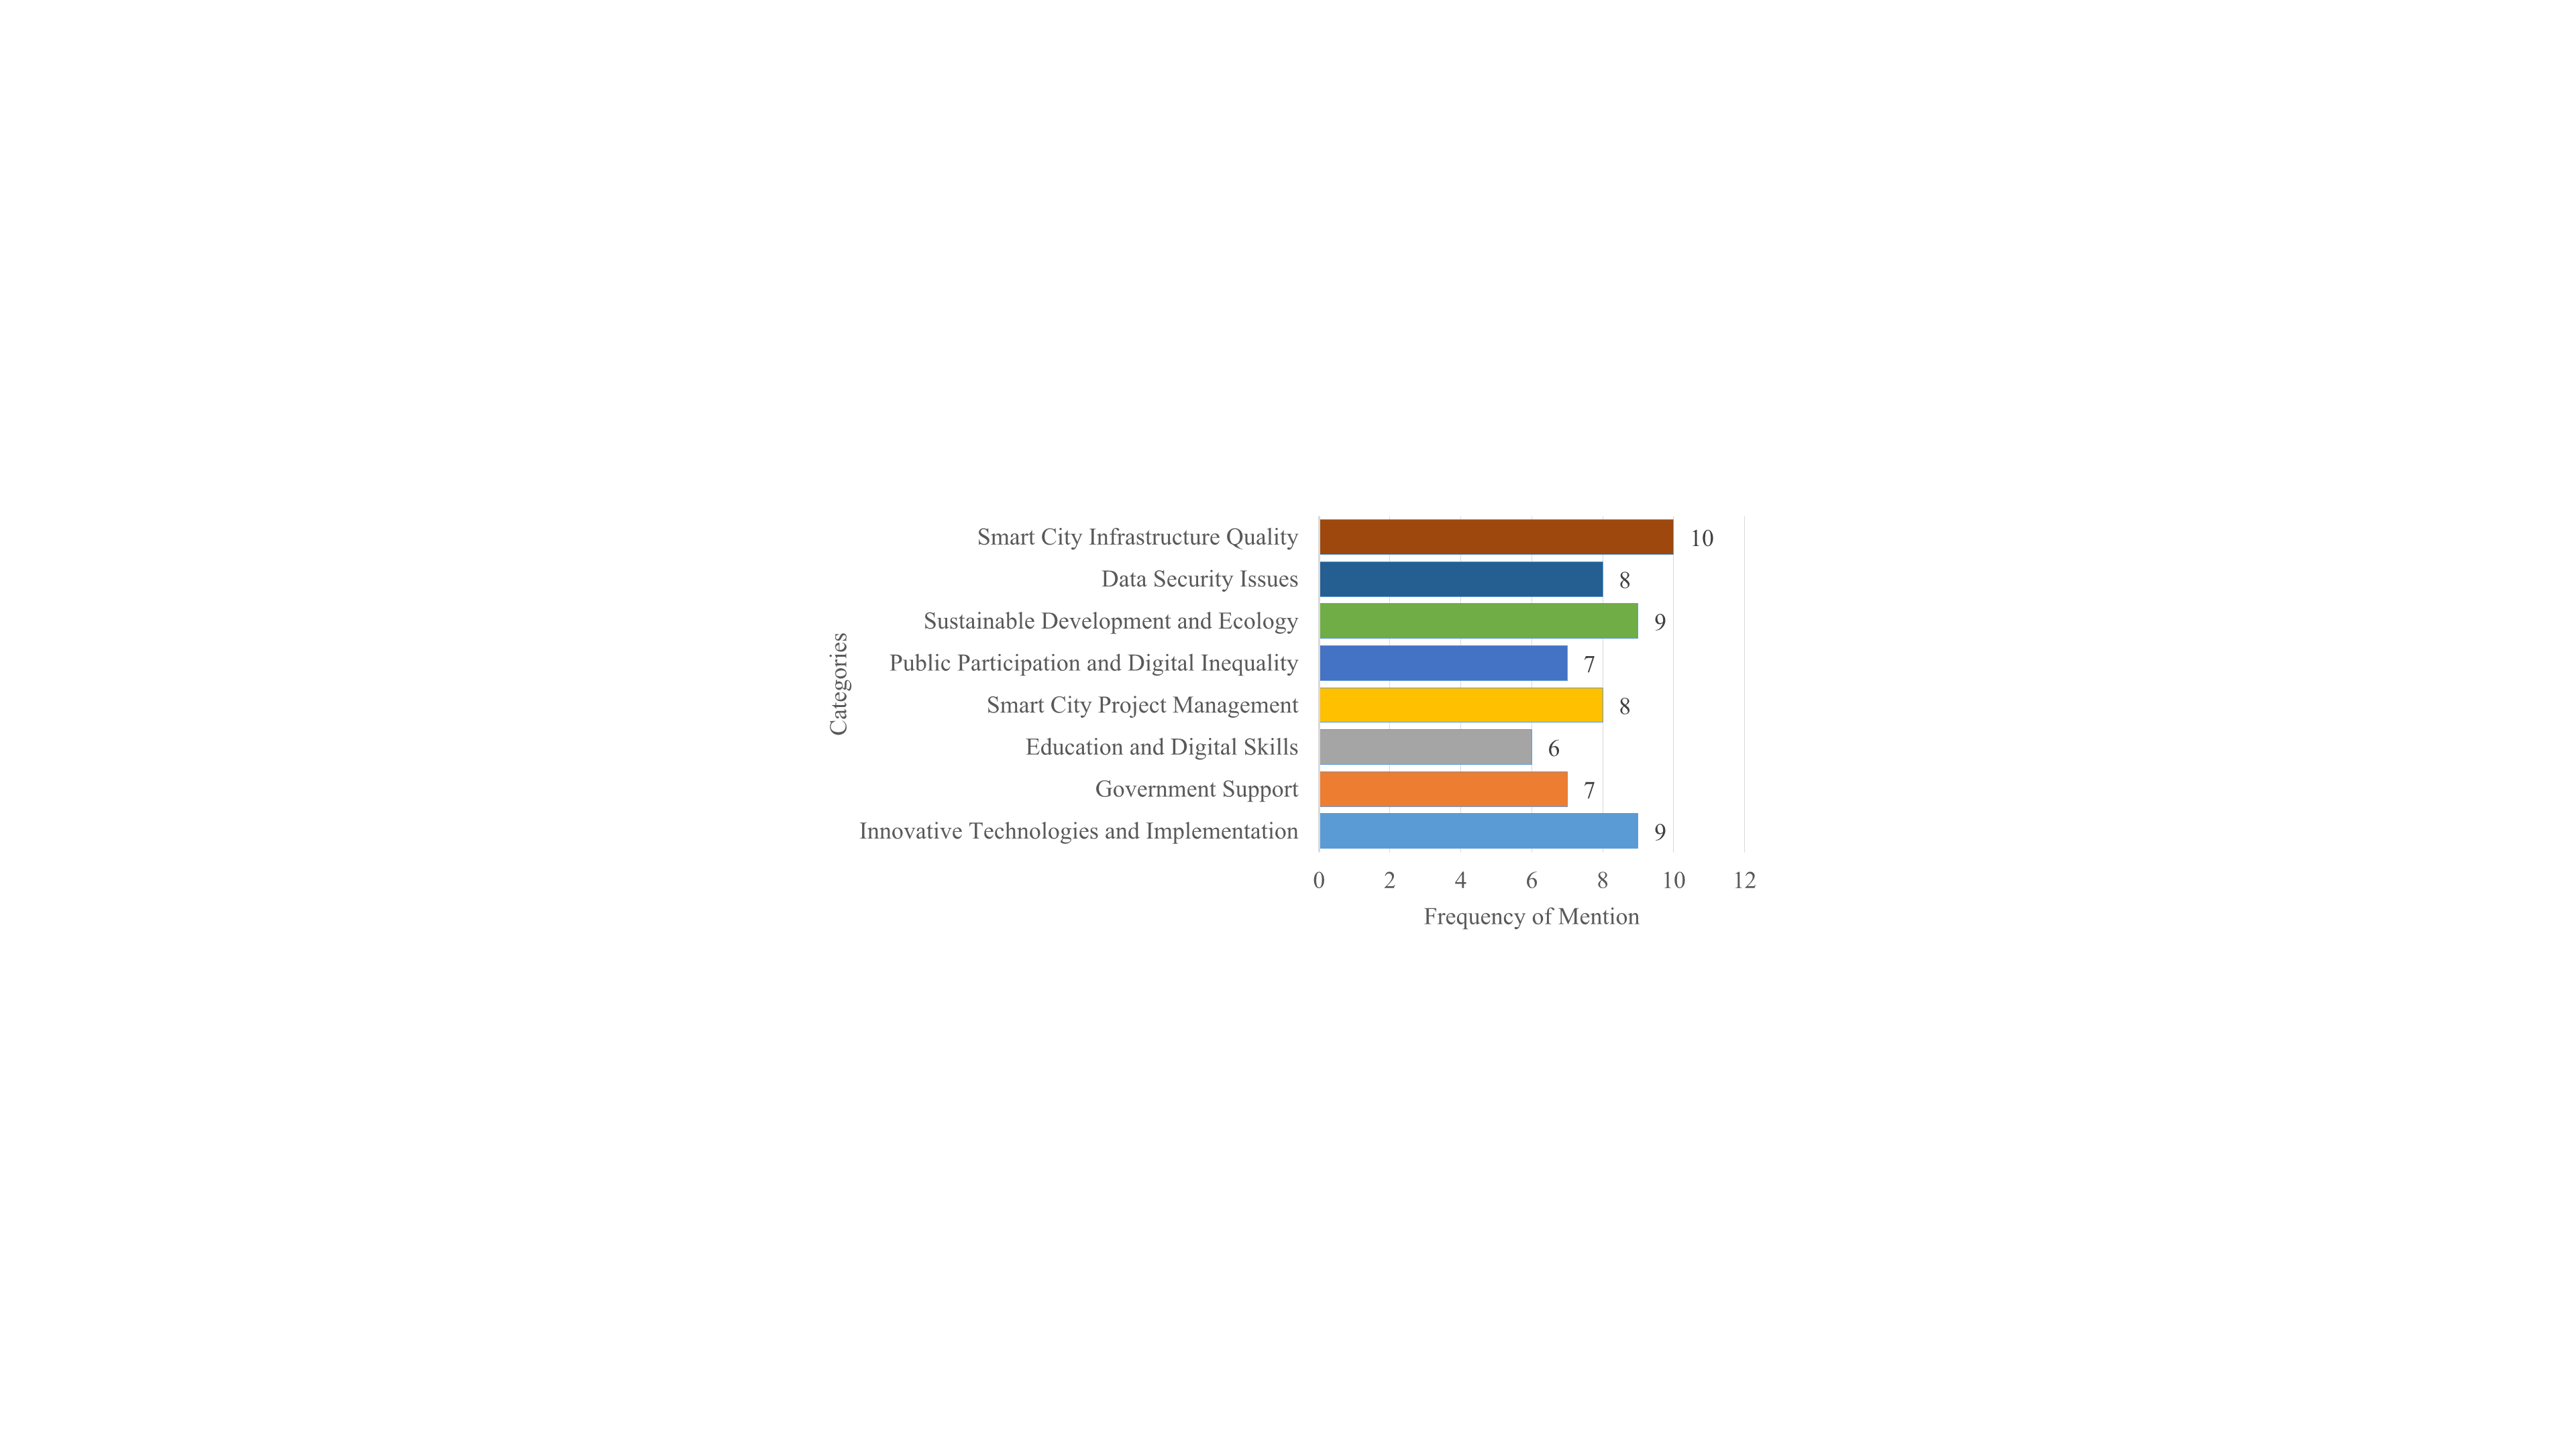
\includegraphics[width=0.8\textwidth]{media/ekon/Graph_15}
	\caption*{Fig. 4 - Frequency of mentions of various key categories related to the development of smart cities}
	\caption*{\normalfont \emph{(compiled by the authors based on {[}28{]})}}
\end{figure}

\begin{multicols}{2}
\emph{Smart City Project Management:}

The mention of project management suggests that effective management
strategies are needed for the successful implementation of smart city
projects, especially when integrating innovative technologies and
coordinating between different sectors.

\emph{Government support:}

Government support plays an important role in the development of smart
cities, including the creation of regulatory norms, financing and
promotion of public-private partnerships. Without stable government
support, such projects are difficult to implement and maintain for a
long time.

\emph{Innovative technologies and their implementation:}

The mention of innovative technologies confirms the importance of using
advanced technologies such as artificial intelligence, big data and the
Internet of Things to solve urban problems. However, their successful
implementation requires careful adaptation to local conditions and
effective application.

\emph{Education and digital skills (A less frequently mentioned
category):}

Interestingly, education and digital skills are mentioned less
frequently, which may indicate that although technology plays an
important role, there is a certain gap in the field of digital literacy
of the population. Providing the necessary training for the workforce
and citizens is critical for the successful implementation of smart city
technologies.

The graph illustrates that the key challenges in the development of
smart cities in Kazakhstan are focused on infrastructure, sustainable
development and data security. However, there are also areas that
require more attention, such as education and digital inequality. These
findings can serve as a basis for future policy decisions and research
aimed at a more balanced and inclusive approach to smart city
development.

Within the framework of the study on the problems and opportunities of
smart city project management using the example of the transformation of
cities in Kazakhstan, several key aspects were analyzed, including
infrastructure quality, sustainable development, data security issues,
public participation, project management and government support. Both
qualitative and quantitative data presented in the form of tables,
graphs and diagrams were used to interpret the results.

\emph{1. The quality of the smart city infrastructure}
\end{multicols}

\begin{table}[H]
\caption*{Table 1 - Frequency of mentioning factors related to infrastructure quality}
\centering
\begin{tblr}{
  row{1} = {c},
  cell{2}{2} = {c},
  cell{3}{2} = {c},
  cell{4}{2} = {c},
  cell{5}{2} = {c},
  hlines,
  vlines,
}
Category                                  & Frequency of mention \\
Transport systems                         & 35                   \\
Energy supply and energy saving           & 28                   \\
Water supply and sanitation               & 22                   \\
Smart buildings and residential complexes & 18                   
\end{tblr}
\end{table}

\begin{table}[H]
\caption*{Table 2 - Frequency of mentioning data security issues in smart cities}
\centering
\begin{tblr}{
  row{1} = {c},
  cell{2}{2} = {c},
  cell{3}{2} = {c},
  cell{4}{2} = {c},
  cell{5}{2} = {c},
  hlines,
  vlines,
}
Data security issue           & Frequency of mention \\
Protection of personal data   & 40                   \\
Cyber threats and hacks       & 33                   \\
IoT Infrastructure Protection & 25                   \\
Threats of information leaks  & 22                   
\end{tblr}
\end{table}

\begin{multicols}{2}
We analyzed the frequency of mentioning factors related to
infrastructure quality (Table 1). The greatest attention in the context
of infrastructure quality is paid to transport systems, which is
explained by the need to solve transport problems such as traffic jams
and the lack of environmentally friendly transport. Energy supply and
energy conservation occupy the second place, due to the growing interest
in sustainable and energy efficient solutions in cities.

\emph{2. Sustainable development and ecology}

Sustainable development is an important topic in the development of
smart cities, which is confirmed by the high frequency of mentioning
environmental technologies. The greatest attention is paid to the
introduction of green technologies, such as solar panels and waste
recycling systems. This is also due to the need to minimize the impact
on the environment in conditions of rapid population growth and
urbanization.

\emph{3. Data security issues}

The list of data security issues in smart cities with their frequency of
mention are presented in Table 2. Data security issues are central to
the challenges faced by smart cities. The protection of
citizens'{} personal data is especially important, which
is becoming critical due to the increased use of the Internet of Things
(IoT) and the collection of big data. Problems with cyber threats and
infrastructure protection also require increased attention, given the
vulnerability of digital systems in smart cities.

\emph{4. Public participation and digital inequality}

Public participation and digital inequality are important aspects in the
management of smart city projects. It is important to ensure access to
technology for all segments of the population in order to avoid a
widening digital divide. The high frequency of mentioning these issues
indicates the need to create inclusive and accessible solutions for all
citizens.

\emph{5. Smart City Project Management}
\end{multicols}

\begin{table}[H]
\caption*{Table 3 - Frequency of mentioning project management issues}
\centering
\begin{tblr}{
  row{1} = {c},
  cell{2}{2} = {c},
  cell{3}{2} = {c},
  cell{4}{2} = {c},
  cell{5}{2} = {c},
  hlines,
  vlines,
}
The problem of project management        & Frequency of mention \\
Coordination between sectors             & 38                   \\
Lack of qualified personnel              & 30                   \\
Development of implementation strategies & 25                   \\
Risk and cost assessment                 & 20                   
\end{tblr}
\end{table}

\begin{table}[H]
\caption*{Table 4 - Frequency of mentioning innovative technologies}
\centering
\begin{tblr}{
  row{1} = {c},
  cell{2}{2} = {c},
  cell{3}{2} = {c},
  cell{4}{2} = {c},
  cell{5}{2} = {c},
  hlines,
  vlines,
}
Innovative technology                        & Frequency of mention \\
Artificial intelligence and machine learning & 45                   \\
Big Data and Analytics                       & 40                   \\
Internet of Things (IoT)                     & 35                   \\
Smart sensors and monitoring                 & 30                   
\end{tblr}
\end{table}

\begin{multicols}{2}
The main challenge in managing smart city projects is coordination
between different sectors such as transport, energy, ecology and
security (Table 3). The lack of qualified personnel and the lack of
clear technology implementation strategies also play a significant role
in the successful implementation of such projects.

\emph{6. Government support}

Government support plays an important role in the successful
implementation of smart city projects. In particular, financing,
regulatory creation and support for public-private partnerships play a
crucial role. The emergence of new forms of government support, such as
subsidies for environmental technologies or tax incentives for
start-ups, contributes to the acceleration of digitalization processes.

\emph{7. Innovative technologies and their implementation}

Innovative technologies play a key role in creating smart cities.
According to Table 4, the greatest attention is paid to artificial
intelligence and machine learning, which make it possible to effectively
manage resources and make decisions based on big data analysis. The
Internet of Things (IoT) is also an integral part of smart cities,
creating a network of connected devices for data collection and
processing.

Kazakhstan' s Energy consumption that comes from
renewables {[}28{]}{\bfseries .} The information supplied about
Kazakhstan' s principal energy contributions from nuclear
and renewable sources has important ramifications for the growth of
smart cities. Figure 5 shows the dynamics of
Kazakhstan' s Energy consumption that comes from
renewables since 1985. Renewable energy has demonstrated a more dynamic
trajectory, whereas nuclear energy has played a minor role, with minimal
contributions throughout the early 1990s and total absence after 1999.
The percentage of renewables started out slowly in 1985 at 1.94\%,
reached a peak of 6.12\% in 2002, and then fluctuated before stabilizing
at 4.52\% in 2023.
\end{multicols}

\begin{figure}[H]
	\centering
	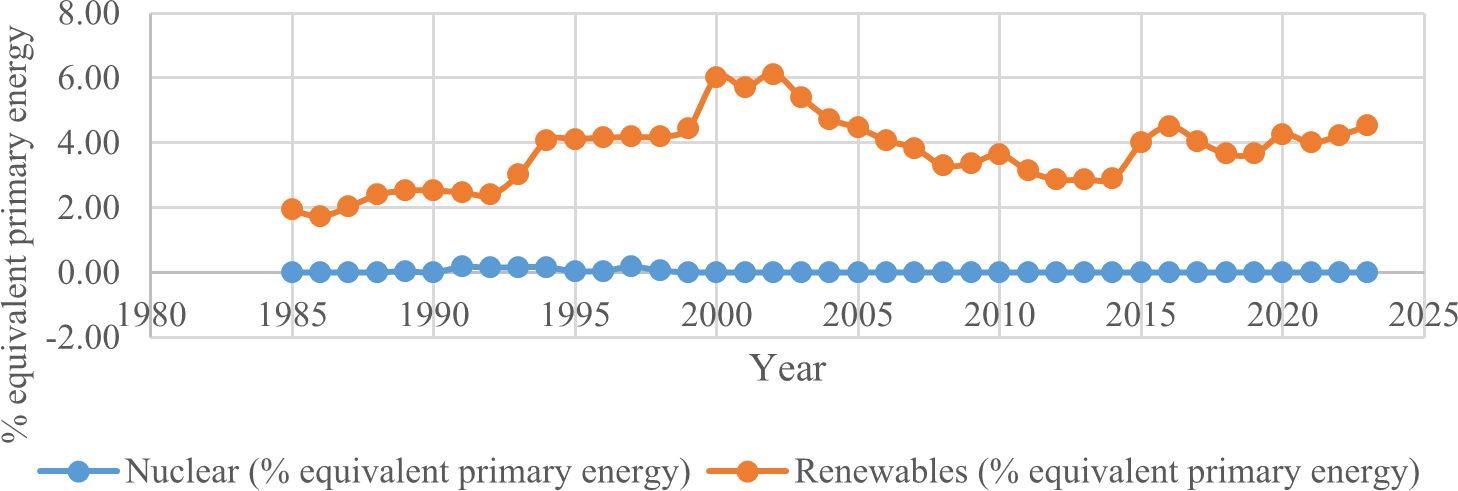
\includegraphics[width=0.75\textwidth]{media/ekon/Graph_16}
	\caption*{Fig. 5 - Kazakhstan' s Energy consumption that comes from renewables}
	\caption*{\normalfont \emph{(compiled by the authors based on {[}28{]})}}
\end{figure}

\begin{multicols}{2}
The growing focus on renewable energy is a crucial component of smart
cities, which place a high priority on sustainability, energy
efficiency, and low-carbon solutions. The 2002 peak points to early
investments in renewable energy, which may have been prompted by
legislative measures or advances in technology. The ensuing drop and
patchy expansion, however, point to difficulties in growing and
maintaining renewable infrastructure, maybe as a result of financial or
regulatory limitations.

The success of Kazakhstan' s smart cities depends on a
more comprehensive and varied energy plan. Energy efficiency and
dependability may be improved by incorporating cutting-edge technology
like smart grids, IoT-based energy management, and AI-driven renewable
forecasting. Furthermore, the lack of nuclear energy represents a lost
chance for reliable, low-carbon baseload electricity that might be used
in conjunction with renewable energy sources in a smart city framework.

In the future, Kazakhstan' s cities must make steady
investments in renewable energy a top priority while investigating
cutting-edge options like decentralized energy generation and energy
storage systems. By lowering reliance on fossil fuels and ensuring a
robust and sustainable energy base, these actions would support global
smart city goals.
\end{multicols}

\begin{center}
{\bfseries Table 5 - Share of various energy sources in Kazakhstan}
\end{center}
\vspace{-1em}
\begin{longtblr}[
  label = none,
  entry = none,
]{
  cells = {c},
  hlines,
  vlines,
}
Year & {Nuclear\\(\% equivalent\\primary\\energy)} & {Renewables\\(\% equivalent\\primary\\energy)} & {Fossil fuels\\(\% equivalent\\primary\\energy)} \\
1985 & 0.00                                        & 1.94                                           & 98.06                                            \\
1986 & 0.00                                        & 1.74                                           & 98.26                                            \\
1987 & 0.00                                        & 2.04                                           & 97.96                                            \\
1988 & 0.00                                        & 2.40                                           & 97.60                                            \\
1989 & 0.03                                        & 2.54                                           & 97.43                                            \\
1990 & 0.00                                        & 2.53                                           & 97.47                                            \\
1991 & 0.18                                        & 2.48                                           & 97.34                                            \\
1992 & 0.16                                        & 2.40                                           & 97.45                                            \\
1993 & 0.17                                        & 3.02                                           & 96.82                                            \\
1994 & 0.16                                        & 4.07                                           & 95.77                                            \\
1995 & 0.04                                        & 4.11                                           & 95.85                                            \\
1996 & 0.05                                        & 4.16                                           & 95.79                                            \\
1997 & 0.19                                        & 4.18                                           & 95.63                                            \\
1998 & 0.06                                        & 4.19                                           & 95.75                                            \\
1999 & 0.00                                        & 4.46                                           & 95.54                                            \\
2000 & 0.00                                        & 6.02                                           & 93.98                                            \\
2001 & 0.00                                        & 5.70                                           & 94.30                                            \\
2002 & 0.00                                        & 6.12                                           & 93.88                                            \\
2003 & 0.00                                        & 5.38                                           & 94.62                                            \\
2004 & 0.00                                        & 4.73                                           & 95.27                                            \\
2005 & 0.00                                        & 4.46                                           & 95.54                                            \\
2006 & 0.00                                        & 4.07                                           & 95.93                                            \\
2007 & 0.00                                        & 3.83                                           & 96.17                                            \\
2008 & 0.00                                        & 3.30                                           & 96.70                                            \\
2009 & 0.00                                        & 3.38                                           & 96.62                                            \\
2010 & 0.00                                        & 3.64                                           & 96.36                                            \\
2011 & 0.00                                        & 3.13                                           & 96.87                                            \\
2012 & 0.00                                        & 2.87                                           & 97.13                                            \\
2013 & 0.00                                        & 2.88                                           & 97.12                                            \\
2014 & 0.00                                        & 2.92                                           & 97.08                                            \\
2015 & 0.00                                        & 4.00                                           & 96.00                                            \\
2016 & 0.00                                        & 4.51                                           & 95.49                                            \\
2017 & 0.00                                        & 4.05                                           & 95.95                                            \\
2018 & 0.00                                        & 3.66                                           & 96.34                                            \\
2019 & 0.00                                        & 3.66                                           & 96.34                                            \\
2020 & 0.00                                        & 4.26                                           & 95.74                                            \\
2021 & 0.00                                        & 4.01                                           & 95.99                                            \\
2022 & 0.00                                        & 4.23                                           & 95.77                                            \\
2023 & 0.00                                        & 4.52                                           & 95.48                                            
\end{longtblr}

\begin{multicols}{2}
The information on Kazakhstan' s energy mix (Table 5)
that has been supplied emphasizes the country' s heavy
reliance on fossil fuels and its gradual decline over time, highlighting
both the opportunities and significant obstacles in the
country' s transition to sustainable energy systems for
the development of smart cities. Up until the early 2000s, fossil fuels
continuously supplied more than 95\% of the equivalent primary energy,
reaching a high of 98.26\% in 1986. During the same time span, fossil
fuel dependence decreased slightly to 93.88\%, while renewable energy
contributions climbed steadily from 1.94\% in 1985 to 6.12\% in 2002.
Since then, the percentage of fossil fuels has remained dominant,
dropping just marginally to 95.48\% in 2023.

Fossil fuel dependence presents serious sustainability issues for smart
cities, such as resource depletion, air pollution, and greenhouse gas
emissions. Reducing reliance on fossil fuels is crucial because smart
cities seek to use cutting-edge technologies to maximize energy
efficiency and make the switch to low-carbon systems. The data shows
that although there has been some progress in integrating renewable
energy, it has not happened quickly enough to significantly reduce
dependency on fossil fuels.

The following are important tactics for smart cities to hasten the
elimination of fossil fuels:

1. Improved Renewable Integration: Reliance on fossil fuels can be
decreased by increasing the use of renewable energy sources including
solar, wind, and hydroelectric power in conjunction with cutting-edge
energy storage systems.

2. Energy Efficiency Measures: To maximize energy use, smart cities can
implement smart grids, IoT-based systems, and energy-efficient
technologies.

3. Policy and Incentives: Strict laws governing the use of fossil fuels,
tax breaks, and subsidies are some ways that governments might
encourage the growth of renewable energy.

4. Public Awareness and Participation: Promoting renewable energy
adoption and lowering dependency on practices that heavily rely on
fossil fuels.

The information emphasizes how urgently strategic actions are needed to
hasten Kazakhstan' s energy transformation. As centers of
sustainability and innovation, smart cities must spearhead this shift by
putting in place comprehensive, tech-driven solutions that allow for a
substantial and long-term decrease in reliance on fossil fuels while
increasing the proportion of renewable energy in the energy mix.

Mobile cellular subscriptions in Kazakhstan {[}9{]}

A key component of the creation of smart cities is the use of mobile
cellular technologies. The trend of mobile cellular subscribers per 100
population in Kazakhstan between 1960 and 2022 demonstrates a
significant shift and underscores the vital role that telecoms play in
promoting digital infrastructure for smart city projects (Figure 6).

A figure of 0.00 per 100 people indicates that Kazakhstan had no mobile
cellular subscriptions between 1960 and 1994. During this time, the
Soviet Union' s centralized system of fixed-line
telephones constituted the majority of the country' s
communication infrastructure. The absence of mobile technology draws
attention to the early phases of digital connectivity, which prepared
the way for later developments in telecommunications.
\end{multicols}

\begin{figure}[H]
	\centering
	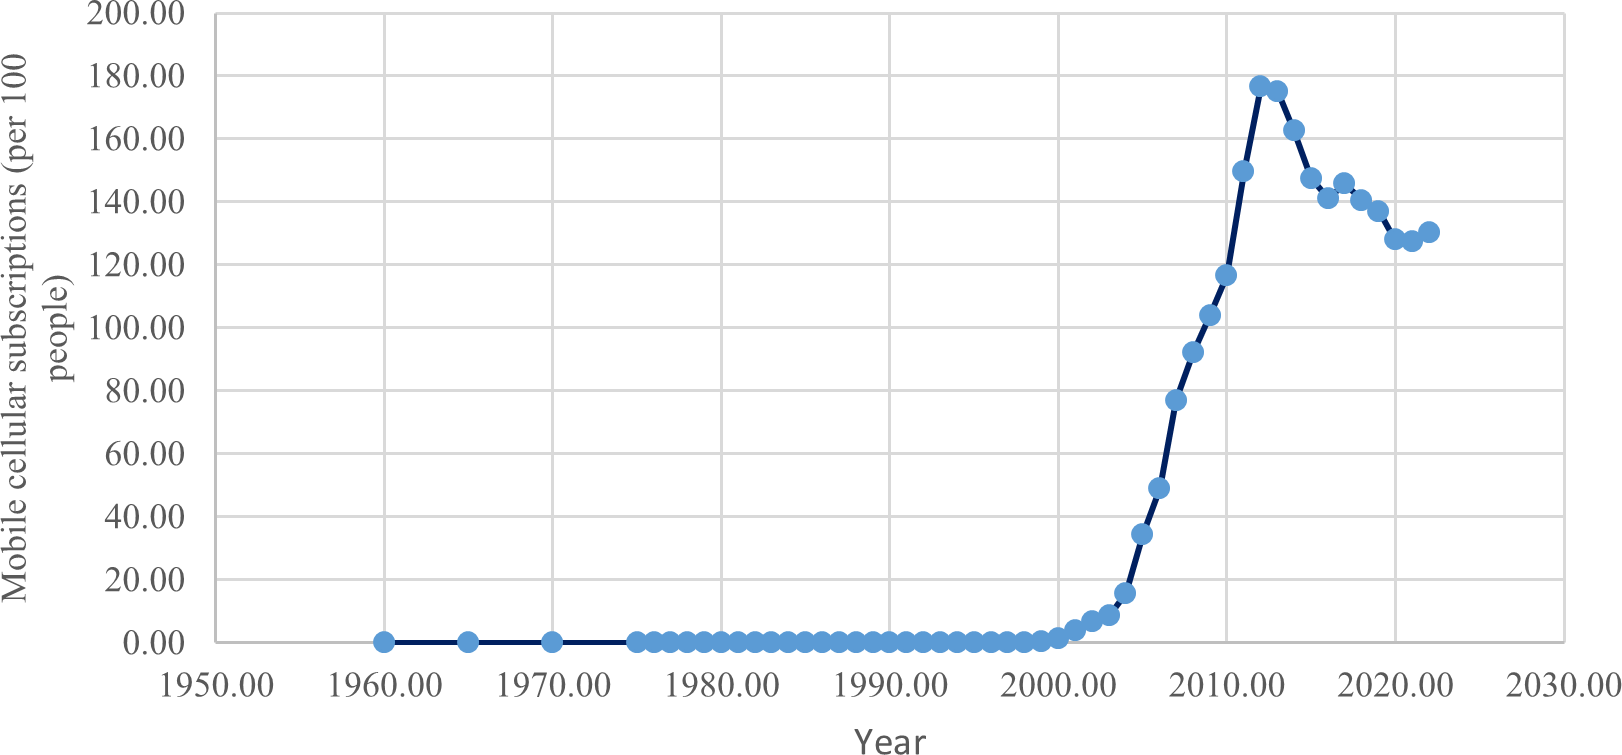
\includegraphics[width=0.75\textwidth]{media/ekon/Graph_17}
	\caption*{Fig.6 - Mobile Cellular subscriptions in Kazakhstan}
	\caption*{\normalfont \emph{(compiled by the authors based on {[}28{]})}}
\end{figure}

\begin{multicols}{2}
A significant change occurred with the advent of mobile cellular
technology in 1995; by 2003, the subscription rate had risen steadily
from 0.03 per 100 persons to 8.63. Initial investments in mobile
infrastructure and the steady uptake of mobile devices are responsible
for this increase. During this time, basic connectivity, a crucial need
for the development of smart cities, particularly in metropolitan areas
was made possible by mobile technology.

Mobile subscriptions increased exponentially between 2004 and 2012,
rising from 15.76 to a peak of 176.79 per 100 persons. Technological
developments, the introduction of 2G and 3G networks, and telecom
carriers'{} aggressive pricing strategies are all
responsible for this quick uptake. Real-time communication, data
exchange, and the establishment of digital services were made possible
by the increase in mobile connectivity, which made Kazakhstani cities
attractive targets for smart city projects. The extensive use of mobile
devices, which are essential for Internet of Things (IoT) applications
in smart city sectors including transportation, energy, and governance,
is reflected in high subscription rates.

By 2022, the subscription rate had marginally decreased from its peak in
2012 to 130.42 per 100 individuals, indicating market saturation and the
rationalization of numerous subscriptions. The penetration rate held
steady in spite of this drop, demonstrating Kazakhstan' s
preparedness for cutting-edge digital solutions. The decrease is in
keeping with the global trend toward integrated communication systems,
where mobile networks support smart city technologies by enhancing Wi-Fi
and internet.

One of the main factors facilitating smart city initiatives in
Kazakhstan is the country' s high rate of mobile
penetration. IoT solutions, such as e-governance platforms, intelligent
transportation systems, and smart metering, are made possible by mobile
networks in smart cities. According to the trends shown, Kazakhstani
cities are in a good position to embrace these technologies, taking use
of the widespread use of mobile devices to link people, companies, and
government services.

Even though mobile connectivity is a major factor in smart city
programs, issues including digital literacy, rural-urban connectivity
gaps, and infrastructure upgrades to 5G networks still exist. The modest
drop in subscription prices over the past few years also points to the
necessity of diversifying digital services in order to keep users
interested. There are opportunities to use mobile networks for smart
city applications, especially in the fields of public services (e.g.,
e-health and e-education), energy (e.g., smart grids), and
transportation (e.g., traffic management).

It will be crucial to integrate mobile cellular networks with
cutting-edge technologies like 5G, AI, and IoT as Kazakhstan moves
forward with its smart city goal. To guarantee fair access to the
advantages of smart cities, policymakers should give mobile
infrastructure improvements top priority, especially in rural areas with
poor connectivity. Furthermore, encouraging public-private
collaborations can help achieve socioeconomic and environmental
objectives while hastening the implementation of smart city solutions.

\emph{ICT Technology adoption-per-100-people in Kazakhstan}

The rapid advancement of mobile cellular technology defined the 2000s
(Figure 7). In 2012, mobile subscriptions reached a peak of 176.79 per
100 individuals, indicating the quick uptake of 2G and 3G networks.
During this decade, internet usage also increased, and by 2012, it had
surpassed 61\% of the population. Despite being adopted more slowly than
mobile services, fixed broadband grew steadily, reaching 12.21 per 100
by 2014.

With mobile cellular subscriptions stable between 127 and 147 per 100
persons, signifying market saturation, the ICT sector developed starting
in 2015. In the meantime, internet penetration reached a remarkable
92.3\% of the population, and fixed broadband subscribers increased to
15.35 per 100 persons by 2022. This illustrates how Kazakhstan is
becoming more and more dependent on broadband internet in order to get
improved digital services.

The steady increase in internet usage demonstrates how well Kazakhstan
has incorporated ICT into daily life, thanks to developments in
broadband and mobile infrastructure. The country is well-positioned to
use ICT for greater digital transformation as it continues to embrace
it, bolstering projects like e-governance, smart cities, and an
increasingly digital economy.
\end{multicols}

\begin{figure}[H]
	\centering
	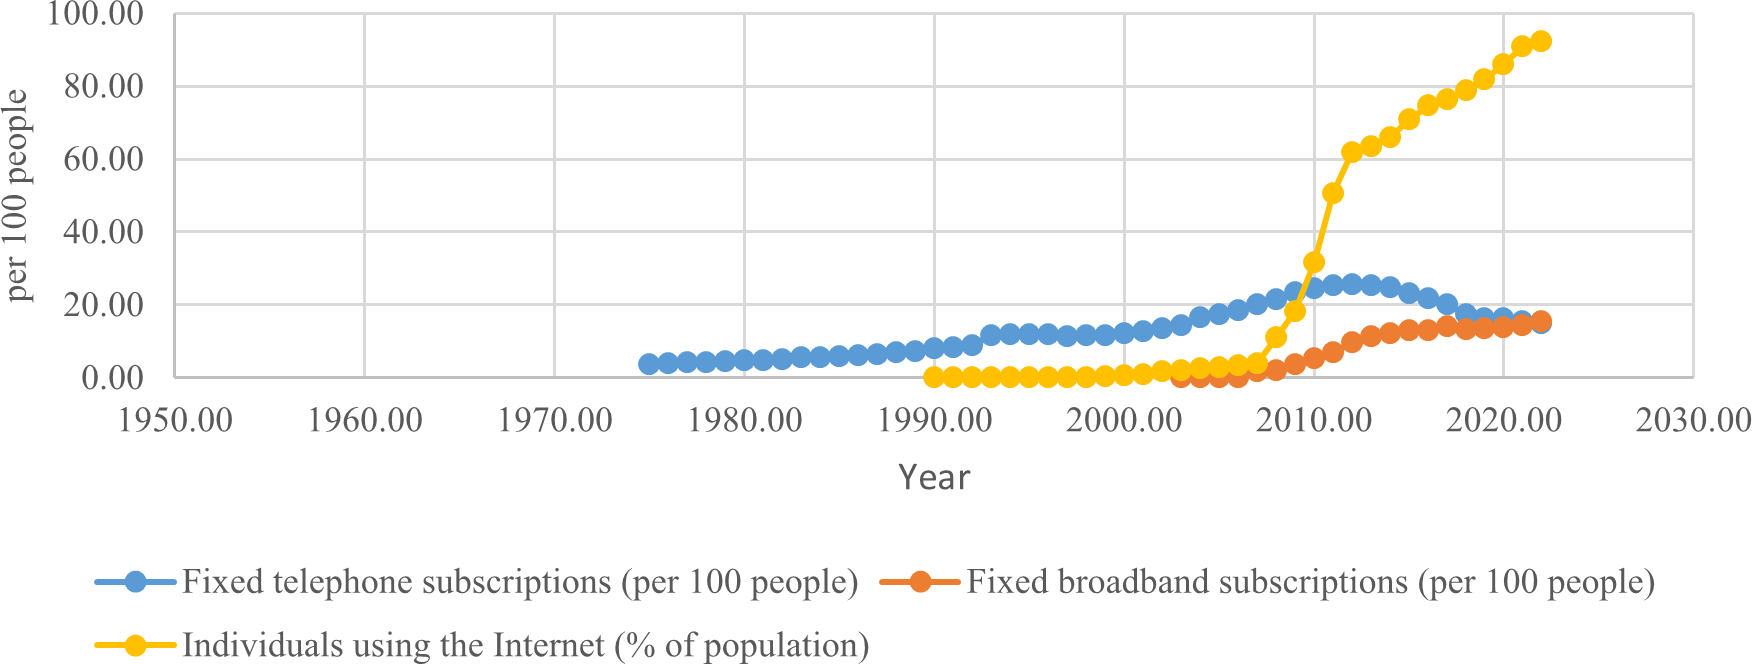
\includegraphics[width=0.75\textwidth]{media/ekon/Graph_18}
	\caption*{Figure 7 - ICT Technology adaptation in Kazakhstan}
	\caption*{\normalfont \emph{(compiled by the authors based on {[}28{]})}}
\end{figure}

\begin{multicols}{2}
Comparing the results obtained with international experience, it can be
noted that Kazakhstan is at the stage of active implementation of its
projects similar to those of other developing countries, however, thanks
to programs such as Digital Kazakhstan, the country has already begun to
successfully solve many of these problems. It is expected that in the
future, increased government funding and the introduction of innovative
technologies, combined with international cooperation, will help
accelerate this process.

{\bfseries Conclusion} Based on the conducted research of problems and
opportunities in the management of smart city projects, several
important conclusions can be drawn on the example of the transformation
of cities in Kazakhstan. Firstly, the development of smart cities in
Kazakhstan faces a number of key challenges, such as the need to
implement sustainable environmental solutions, ensuring public
participation in the digitalization process, overcoming digital
inequality, as well as the need for government support and the creation
of appropriate regulatory conditions for the implementation of such
projects. These problems turned out to be systemic, requiring an
integrated approach and integration into the existing urban
infrastructure.

Secondly, the results of the study demonstrated a high interest in the
issues of sustainable development and ecology in the design of smart
cities. Environmental aspects such as the use of green technologies,
solar panels, waste recycling and energy conservation occupy an
important place in urban plans. This trend is confirmed by an increase
in the frequency of mentioning environmental aspects in modern design
studies, which also indicates an increasing attention to the issue of
sustainability at the level of public and private initiatives.

Thirdly, despite active efforts on the part of the Government and the
private sector, the challenges of ensuring broad public participation
and eliminating digital inequality remain important obstacles to the
effective introduction of technology into the urban environment. Citizen
participation in the digitalization process requires the creation of
more open platforms for communication and participation in
decision-making, as well as more accessible educational and technical
solutions for all segments of the population. Digital inequality, in
turn, limits citizens'{} access to the latest
technologies, which reduces the overall potential for creating effective
and inclusive smart cities.

\emph{{\bfseries Funding.} This research has been funded by the Committee
of Science of the Ministry of Science and Higher Education of the
Republic of Kazakhstan (Grant No. BR24993051 ``Development of an
intelligent city system based on IoT and data analysis'')}
\end{multicols}

\begin{center}
{\bfseries References}
\end{center}

\begin{references}
1. Tehnologii umnyh gorodov: chto vlijaet na vybor gorozhan?
{[}Electronic resource{]} // McKinsey \& \\Company. -2018. URL:
\href{https://www.mckinsey.com/industries/public-sector/our-insights/smart-city-solutions-what-drives-citizen-adoption-around-the-globe/ru-RU}{https://www.mckinsey.com} . Date
of application: 06.12.2024. {[}in Russian{]}

2. Worldwide Spending on Public Cloud Services is Forecast to Reach
\$1.35 Trillion in 2027, According to New IDC Spending Guide
{[}Electronic resource{]} // IDC. -2023. URL:
\href{https://www.idc.com/getdoc.jsp?containerId=prUS51179523}{https://www.idc.com} . Date
of application: 12.12.2024.

3. Cities Across Central Asia Can Unlock Full Economic Potential by
Implementing Low-Carbon and Climate-Resilient Development Strategies,
{[}Electronic resource{]} //World bank group. -2023. URL\\
\href{https://www.worldbank.org/en/news/press-release/2023/09/27/cities-across-central-asia-can-unlock-full-economic-potential-by-implementing-low-carbon-development-strategies}{https://www.worldbank.org}
Date of application 10.12.2024.

4. Urdabayev M, Kireyeva A, Vasa L, Digel I, Nurgaliyeva K, Nurbatsin A
Discovering smart cities' potential in Kazakhstan: A cluster analysis
// PLoS ONE. -2024. -Vol. 19(3).
\href{https://doi.org/10.1371/journal.pone.0296765}{DOI\\
10.1371/journal.pone.0296765}

5. Camero A., Alba E. Smart City and information technology: A review //
Cities-- 2019. --Vol. 93. - P. 84-94. DOI 10.1016/j.cities.2019.04.014

6. Cartalis C. Toward resilient cities - a review of definitions,
challenges and prospects // Adv. Build. Energy Res. -2014. -Vol. 8(2).
-P. 259-266. DOI 10.1080/17512549.2014.890533

7. Voytenko Y., Mccormick K., Evans J., Schliwa G. Urban living labs for
sustainability and low carbon cities in Europe: towards a research
agenda // J. Clean. Prod. -2016. -Vol. 123. -P. 45-54. DOI\\
10.1016/j.jclepro.2015.08.053

8. Yigitcanlar T., Kamruzzaman M., Foth M., Sabatini-Marques J., da Costa
E., Ioppolo G. Can cities become smart without being sustainable? A
systematic review of the literature // Sustain. Cities Soc. -2019.
-Vol. 45. -P. 348-365. DOI 10.1016/j.scs.2018.11.033

9. Noy K., Givoni M. Is 'smart mobility' sustainable? Examining the views
and beliefs of transport's technological entrepreneurs //
Sustainability. -2018. -Vol. 10(2):422. DOI 10.3390/su10020422

10. Young M., Farber S. Ride-hailing platforms are shaping the future of
mobility, but for whom? // In The Platform Economy and the City: Urban
Peril and Promise in the New Digital Economy / Zwick, A., Spicer, Z.,
Eds. Montreal, QC, Canada: McGill-Queens University Press, 2021. DOI
10.31219/osf.io/pz7fk

11. Verrest H., Pfeffer K. Elaborating the urbanism in smart urbanism:
distilling relevant dimensions for a comprehensive analysis of Smart
City approaches // Inf. Commun. Soc. -2019. -Vol. 22(9). -P.
1328-1342. DOI:10.1080/1369118X.2018.1424921

12. Nguyen H.T., Marques P., Benneworth P. Living labs: Challenging and
changing the smart city power relations?//Technol. Forecast. Soc.
Change.-2022. -Vol. 183.
DOI 10.1016/j.techfore.2022.121866

13. Parygin D., Sadovnikova N., Gamidullaeva L., Finogeev A., Rashevskiy
N. Tools and Technologies for Sustainable Territorial Development in
the Context of a Quadruple Innovation Helix // Sustainability. - 2022.
-Vol. 14(15):9086. DOI 10.3390/su14159086

14. Meijer A., Bolívar M.P.R. Governing the smart city: a review of the
literature on smart urban \\governance // Int. Rev. Adm. Sci. -2016. -Vol.
82(2). -P. 392-408. DOI 10.1177/0020852314564308

15. Ramaswami A., Russell A.G., Culligan P.J., Rahul Sharma K., Kumar E.
Meta-principles for developing smart, sustainable, and healthy cities
// Science. -2016. -Vol. 352(6288). -P. 940-943. DOI\\
10.1126/science.aaf7160

16. Weber-Lewerenz B., Traverso M. Navigating Applied Artificial
Intelligence (AI) in the Digital Era: How Smart Buildings and Smart
Cities Become the Key to Sustainability // Journal of Artificial
Intelligence and Applications. -2023. -Vol. 1(4). -P. 214-227.
DOI \href{http://dx.doi.org/10.47852/bonviewAIA32021063}{10.47852/bonviewAIA32021063}

17. Yigitcanlar T., Kamruzzaman M., Buys L., Ioppolo G., Sabatini-Marques
J., da Costa E.M., Yun J.H.J. Understanding `smart cities':
Intertwining development drivers with desired outcomes in a
multidimensional framework //Cities. -2018. -Vol. 81. -P. 145-160.
DOI 10.1016/J.CITIES.2018.04.003

18. Mora L., Deakin M., Reid A. Combining co-citation clustering and
text-based analysis to reveal the main development paths of smart
cities // Technol. Forecast. Soc. Change. -2019. -Vol. 142. - P.
56-69. DOI 10.1016/j.techfore.2018.07.019

19. Robinson, P.; Coutts, S. 16-The case of Quayside, Toronto, Canada //
In Smart City Emergence; Elsevier: Amsterdam, The Netherlands. -2019.
-P. 333-350. DOI 10.1016/B978-0-12-816169-2.00016-X

20. Yoo, Y., Boland R.J., Lyytinen K., Majchrzak A. Organizing for
innovation in the digitized world // Organ. Sci. -2012. -Vol. 23. -P.
1398-1408. DOI 10.1287/orsc.1120.0771

21. Trindade E.P., Hinnig M.P.F., Costa E.M., Marques J.S., Bastos R.C.,
Yigitcanlar T. Sustainable development of smart cities: a systematic
review of the literature // Journal of Open Innovation: Technology,
Market, and Complexity. - 2017.-Vol.3(3) - P.1-14.
DOI 10.1186/s40852-017-0063-2.

22. Bibri S.E., Krogstie J. Smart sustainable cities of the future: An
extensive interdisciplinary literature review //Sustain. Cities Soc.
-2017. -Vol. 31(25). -P. 183-212.
DOI 10.1016/j.scs.2017.02.016

23. Bibri S.E. On the sustainability of smart and smarter cities in the
era of big data: an interdisciplinary and transdisciplinary literature
review // J. Big Data. -2019. -Vol. 6(1). DOI
10.1186/s40537-019-0182-7

24. Ben Letaifa, S. How to strategize smart cities: Revealing the SMART
model // J. Bus. Res. -2015. -Vol. 68(7). -P. 1414-1419. DOI
10.1016/j.jbusres.2015.01.024

25. Guedes, A.L.A.; Alvarenga, J.C.; Goulart, M.d.S.S.; y Rodriguez,
M.V.R.; Soares, C.A.P. Smart cities: The main drivers for increasing
the intelligence of cities // Sustainability. -2018. --Vol.
10(9):3121. DOI 10.3390/su10093121

26. Veloso, Á., Fonseca, F., \& Ramos, R. Insights from Smart City
Initiatives for Urban Sustainability and Contemporary Urbanism. Smart
Cities. -2024. -Vol. 7(6). -P. 3188-3209. DOI
10.3390/smartcities7060124

27. Giffinger, R., Haindlmaier, G. Benchmarking the Smart City: A Sound
Tool for Policy-Making? // Scienze Regionali. - 2018. - Vol. 17(1).
-P. 115-122. DOI 10.14650/88820.

28. Statistical Review of World Energy {[}Electronic resource{]} //Energy
Institute. -- 2024. URL: \\\href{https://www.energyinst.org/statistical-review}{https://www.energyinst.org}
.Date of application 14.12.2024.
\end{references}

\begin{authorinfo}
\emph{{\bfseries Information about the authors}}

Galymzhanova A.- Doctoral Candidate, Kazakh National University named
after al-Farabi, Almaty, Kazakhstan, e-mail:\\
\href{mailto:aiddaanaa07@gmail.com}{\nolinkurl{aiddaanaa07@gmail.com}};

Singh S.- Ph.D., Professor, University of Fiju, Republic of Fiju,
e-mail:
\href{mailto:satyanand.singh@fnu.ac.fj}{\nolinkurl{satyanand.singh@fnu.ac.fj}};

Sarkambayeva Sh. -Ph.D., Kazakh National Research Technical University
named after K.I. Satpayev, Almaty, \\Kazakhstan, e-mail:
\href{mailto:sh.sarkambayeva@satbayev.university}{\nolinkurl{sh.sarkambayeva@satbayev.university}};

Boranbayeva A. - Ph.D., Kazakh National University named after
al-Farabi, Almaty, Kazakhstan, e-mail: \\boranbaeva7777@gmail.com;

Turegeldinova A. - PhD, Candidate of Economic Sciences, Kazakh National
Research Technical University named after K.I. Satpayev, Almaty,
Kazakhstan, e-mail: a.turegeldinova@satbayev.university

\emph{{\bfseries Сведения об авторах}}

Галымжанова A. - докторант, Казахский национальный университет имени
аль-Фараби, Алматы, Казахстан, e-mail: \\aiddaanaa07@gmail.com;

Сингх С. -Ph.D., профессор, Университет Фиджи, Республика Фиджи, e-mail:
satyanand.singh@fnu.ac.fj;\\

Саркамбаева Ш.Г. - Ph.D., Казахский национальный исследовательский
технический университет им. К.И. Сатпаева, Алматы, Казахстан, e-mail:
sh.sarkambayeva@satbayev.university

Боранбаева A. - Ph.D., Казахский национальный университет имени
аль-Фараби, Алматы, Казахстан, e-mail: \\boranbaeva7777@gmail.com;

Турегельдинова А. - к.э.н., PhD, Казахский национальный
исследовательский технический университет им. К.И. Сатпаева, Алматы,
Казахстан, e-mail:a.turegeldinova@satbayev.university
\end{authorinfo}
